% 6. Empirical Evaluation and Results 
\section{Experimental Design and Performance Evaluation}
\label{ch:experimental_design_and_results}

This chapter details the framework for training and evaluating the trajectory prediction model. It outlines the experimental setup, the learning objectives, and the metrics used for assessment, followed by a quantitative and qualitative analysis of the model's performance.

% 5. subsection: Training and Evaluation Paradigm 
\subsection{Training and Evaluation Paradigm}
\label{sec:training_and_evaluation_paradigm}

The training and evaluation environment uses a robust and reproducible setup. This subsection details the computational environment, configuration management, and the data processing pipeline.

\subsubsubsection{Training Environment and Configuration}
\label{sec:exp_training_env_merged}
% Specification of the computational setup (PyTorch Lightning, WandB for experiment tracking and logging) and critical hyperparameters. 
% Discussion of the rationale behind the selected configurations. 

The entire suite for training, evaluation, and logging is managed through PyTorch Lightning, with experiment tracking and visualization handled by Weights \& Biases (WandB). This setup facilitates managed logging, checkpointing, and distributed training strategies.

All configurations and hyperparameters are managed by Pydantic. This enables a ``Config-as-Factory'' pattern, which simplifies the process of swapping different models, datasets, or loss functions. While the environment is robustly configured, the provided documentation does not detail specific hyperparameters such as batch size or learning rate.

\subsubsubsection{Data Handling and Processing}
\label{sec:data_handling_merged}

For high-throughput data ingestion, the data loading pipeline uses HDF5. The framework enhances processing efficiency by randomly partitioning the full sample index into 32 shards and assigning one shard to each DataLoader worker, which ensures balanced and parallel prefetching.

% - How iterative improvements are achieved during training (e.g. loss on intermediate decoder layers for MTR ). 
The training data undergoes a detailed processing pipeline before being fed to the model:
\begin{itemize}
    \item \textbf{Agent Selection:} First, the pipeline selects agents—vehicles, pedestrians, or cyclists—based on their movement distance and visibility within scenarios.
    \item \textbf{Scenario Classification:} Scenarios receive a difficulty classification (Easy, Medium, Hard) derived from a Kalman filter analysis.
    \item \textbf{Coordinate Normalization:} The system then normalizes all coordinate data into an agent-centric frame using the rotation matrix $R_{z}(-\theta_{c})$.
    \item \textbf{Tensor Assembly:} Finally, it assembles agent and map features into padded and masked tensors, specifically $\mathbb{R}^{N_{max}\times T_{p}\times F_{ap}}$ for dynamic agent data and $\mathbb{R}^{K\times L\times F_{map}}$ for static map data, preparing them for model ingestion.
\end{itemize}

\subsection{Optimization Strategy and Learning Objective}
\label{sec:exp_optimization_merged}

The MTR model was trained from scratch without the use of a pre-trained model. A significant portion of the implementation involved adapting the model to the UniTraj framework's data parsing and configuration systems.
% - The overall objective the model is trained to optimize. 
The primary learning objective is to train the model to accurately forecast multimodal trajectories.

% Detailed specification of the loss function(s) employed for MTR training, including components for trajectory regression and mode probability classification. 
% - Specific loss components and their roles. 
% - e.g., For MTR: Gaussian Regression Loss (NLL) and auxiliary L1 regression loss. 
% - Any specific strategies like hard assignment in MTR. 
% Discussion of how this objective function guides the model to learn multimodal distributions (e.g., relationship to Brier-FDE if incorporated). 
The UniTraj framework unifies loss functions for different models, and the overall training objective is to minimize these functions to improve prediction accuracy. The training process specifically seeks to decrease metrics like the minimum Final Displacement Error (FDE). A key component of the objective is the Brier Final Displacement Error, which assesses both the accuracy of the trajectory's final point and the model's confidence in its prediction. This objective guides the model to learn multimodal distributions. However, the exact mathematical formulation of the loss function used for this training run is not specified in the source material. 
% e.g., Adam optimizer with specified learning rate and scheduling. 
% - Optimizer used, learning rate, batch size, epochs etc. 
Similarly, the specific optimization algorithm, such as Adam or SGD, and its associated parameters like learning rate and scheduling, are not mentioned.

\subsection{Evaluation Metrics}
\label{sec:exp_metrics_merged}

The model's performance assessment relies on a set of standard industry metrics. The mathematical definitions for these metrics are as follows:
\begin{itemize}
    \item \textbf{Average Displacement Error (ADE):} The mean L2 distance between the predicted trajectory and the ground truth across all time steps, defined as $ADE=\mathbb{E}_{t}[||\hat{y}_{t}-y_{t}||_{2}]$.
    \item \textbf{Final Displacement Error (FDE):} The L2 distance between the final predicted position and the ground truth final position, given by $FDE=||\hat{y}_{T}-y_{T}||_{2}$.
    \item \textbf{Miss Rate (MR):} The fraction of predictions where the FDE for the most likely trajectory exceeds a distance threshold $d_{thresh}$ (e.g., 2.0 m). The formula is $MR=\mathbb{E}_{k}[\mathbb{I}\{||\hat{y}_{T}^{(k)}-y_{T}||_{2}>d_{thresh}\}]$.
    \item \textbf{Brier Final Displacement Error (BrierFDE):} A metric that scores both trajectory accuracy and its assigned probability, defined as $BrierFDE=\mathbb{E}_{k}[p_{k}\cdot||\hat{y}_{T}^{(k)}-y_{T}||_{2}^{2}]$.
\end{itemize}

\subsection{Performance Analysis}
\label{sec:performance_analysis_merged}
This subsection evaluates the trained MTR model's performance through quantitative metrics and qualitative review. The analysis confirms the model's learning effectiveness and its ability to generate accurate and probable trajectory forecasts.

\subsubsubsection{Quantitative Performance Analysis}
\label{sec:results_quantitative_merged}
% Presentation and statistical analysis of validation metrics (brier-minFDE, minFDE, minADE, Miss Rate). 
% Add actual results, tables, figures. 
% Comparison against reported benchmarks (e.g., UniTraj paper results ), with careful consideration of comparability. 

The quantitative analysis of the MTR model's performance is based on metrics recorded during training and validation. The training process shows a clear reduction in loss values, indicating the model is learning from the data. The plots in Figure \ref{fig:training_metrics_grid_merged} exhibit a characteristic learning curve: a steep reduction in error during initial training, which then gradually plateaus. This trend indicates convergence.

% toDO(luroess): Split graphs for better visualization?
\begin{figure}[htbp]
    \centering
    \begin{subfigure}[b]{0.48\textwidth}
        \centering
        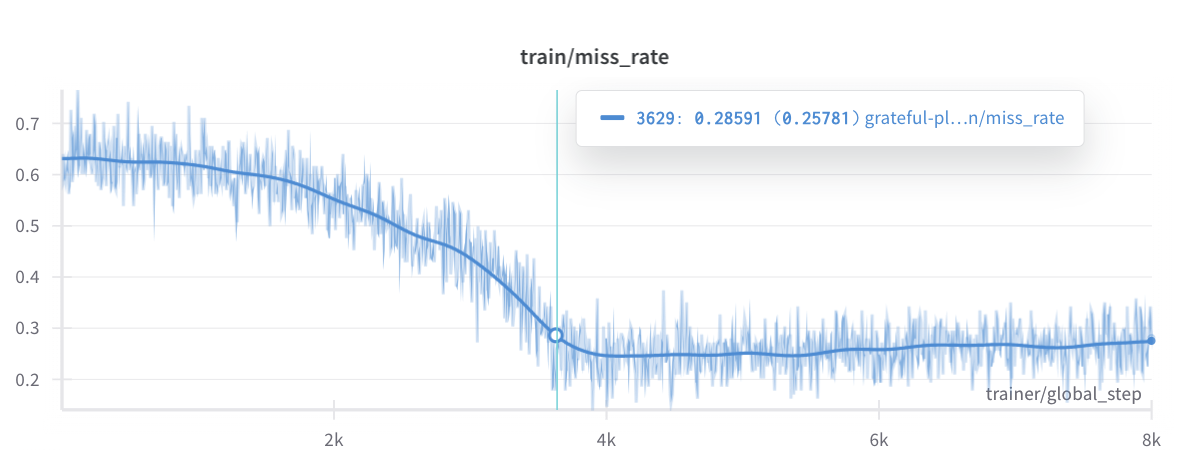
\includegraphics[clip, width=\textwidth]{figures/train_miss_rate.png}
        \caption{train/miss\_rate}
    \end{subfigure}
    \hfill
    \begin{subfigure}[b]{0.48\textwidth}
        \centering
        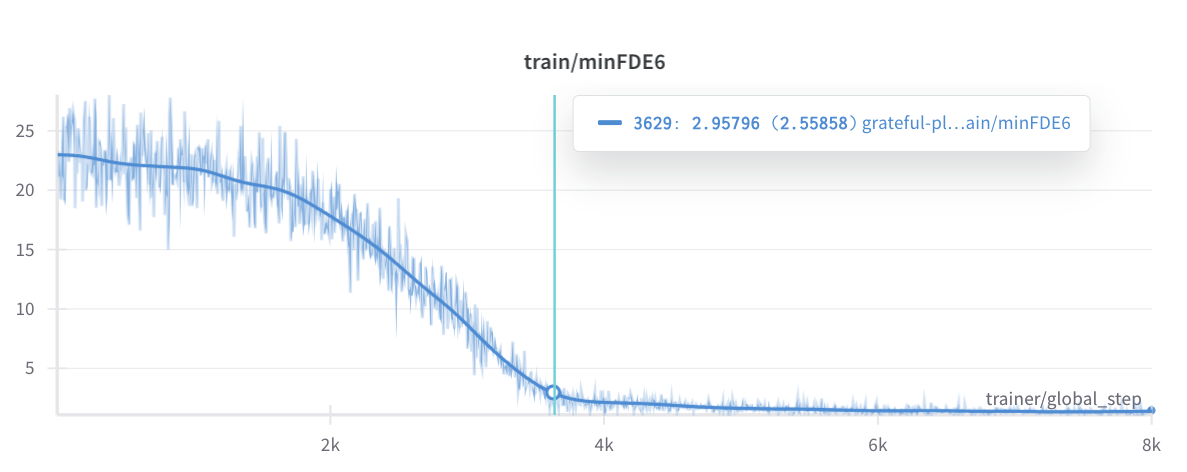
\includegraphics[clip, width=\textwidth]{figures/train_min_fde6.png}
        \caption{train/minFDE6}
    \end{subfigure}
    \vfill
    \begin{subfigure}[b]{0.48\textwidth}
        \centering
        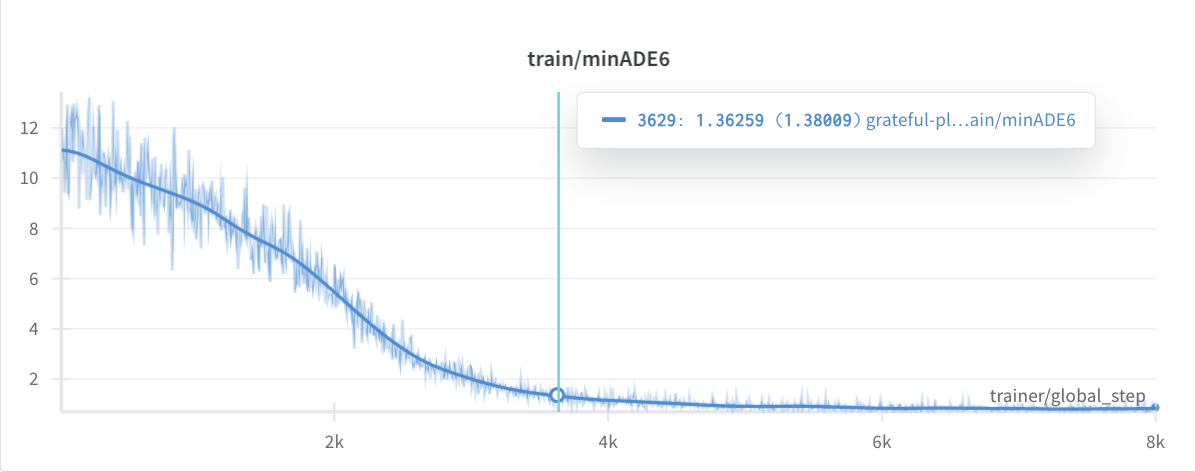
\includegraphics[clip, width=\textwidth]{figures/train_min_ade6.png}
        \caption{train/minADE6}
    \end{subfigure}
    \hfill
    \begin{subfigure}[b]{0.48\textwidth}
        \centering
        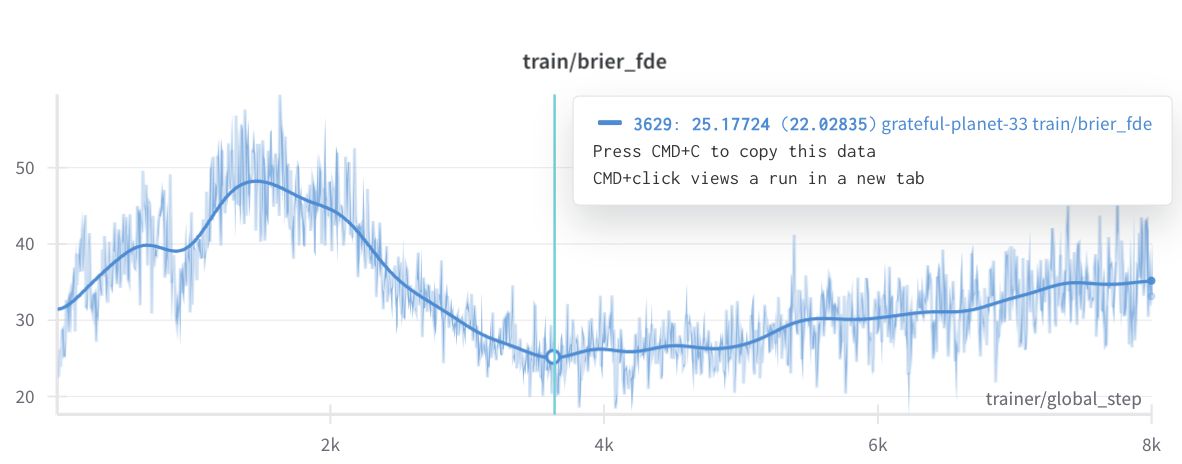
\includegraphics[clip, width=\textwidth]{figures/train_brier_fde.png}
        \caption{train/brier\_fde}
    \end{subfigure}
    \caption{A grid of performance metrics on the training set. The plots show a consistent decrease in error for miss rate, brier FDE, minFDE6, and minADE6 over approximately 6,000 training step of batches, which indicates successful learning. }
    \label{fig:training_metrics_grid_merged}
\end{figure}

Final validation metrics, taken at step 31,295 (6,259 batches), are presented in Table \ref{tab:validation_results}.  On the validation set, the trained MTR model achieved a brier-minFDE of 1.98, a minFDE of 1.6655, a minADE of 0.86294, and a Miss Rate of 0.30141.  These results are comparable to baseline values from existing literature.  The consistent decrease in error seen in Figure \ref{fig:validation_metrics_merged} demonstrates that the model generalizes well to unseen data.  Notably, the Brier-FDE of 1.98 shows a slight improvement over the 2.08 value reported in the MTR paper's appendix, highlighting the effectiveness of this training implementation. 

\begin{table}[htbp]
    \centering
    \caption{Final Validation Metrics at Step 31,295}
    \label{tab:validation_results}
    \begin{tabular}{@{}lcc@{}}
        \toprule
        \textbf{Metric} & \textbf{Value} & \textbf{Benchmark (MTR Paper)} \\
        \midrule
        brier-minFDE & 1.98  & 2.08  \\
        minFDE & 1.6655  & - \\
        minADE & 0.86294  & - \\
        Miss Rate & 0.30141  & - \\
        \bottomrule
    \end{tabular}
\end{table}

% toDO(luroess): Split graphs for better vizualization?
\begin{figure}[htbp]
    \centering
    \begin{subfigure}[b]{0.48\textwidth}
        \centering
        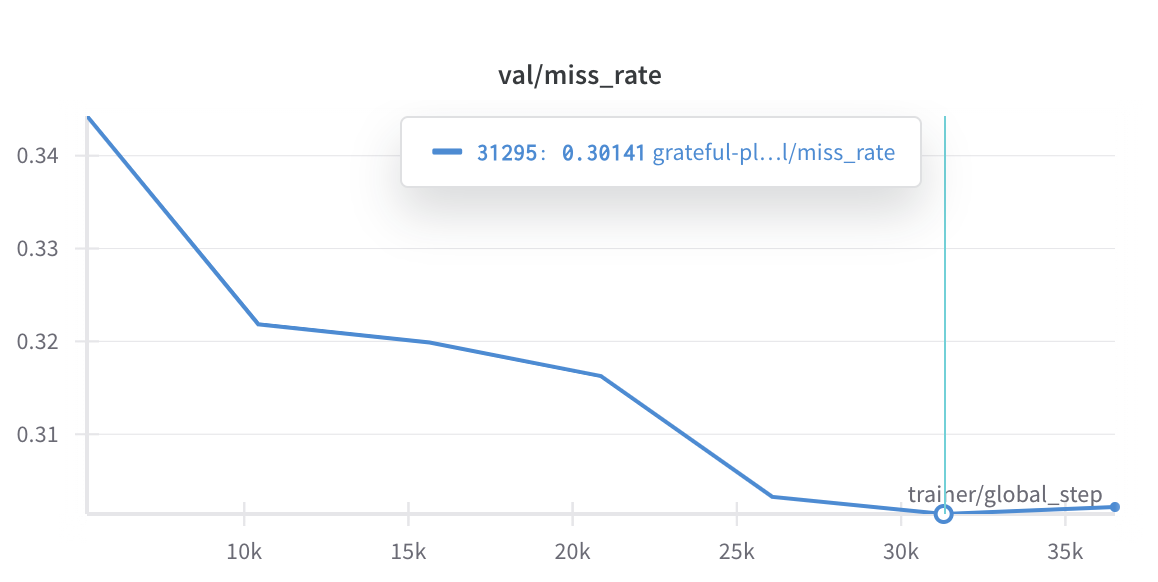
\includegraphics[clip, width=\textwidth]{figures/val_miss_rate.png}
        \caption{val/miss\_rate: 0.30141}
    \end{subfigure}
    \hfill
    \begin{subfigure}[b]{0.48\textwidth}
        \centering
        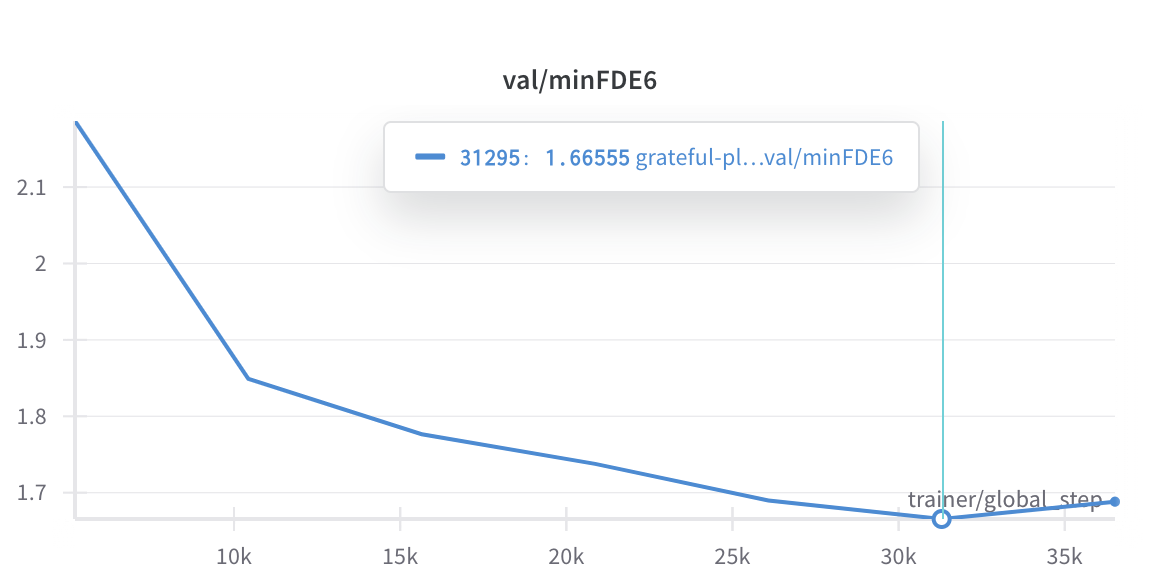
\includegraphics[clip, width=\textwidth]{figures/val_min_fde6.png}
        \caption{val/minFDE6: 1.6655}
    \end{subfigure}
    \vfill
    \begin{subfigure}[b]{0.48\textwidth}
        \centering
        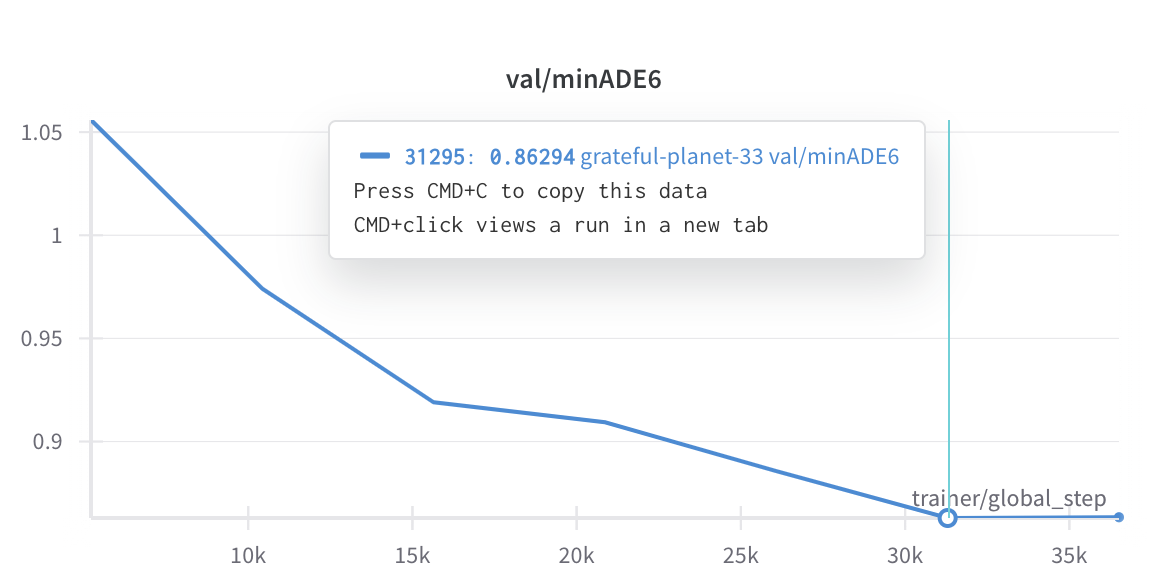
\includegraphics[clip, width=\textwidth]{figures/val_min_ade6.png}
        \caption{val/minADE6: 0.86294}
    \end{subfigure}
    \hfill
    \begin{subfigure}[b]{0.48\textwidth}
        \centering
        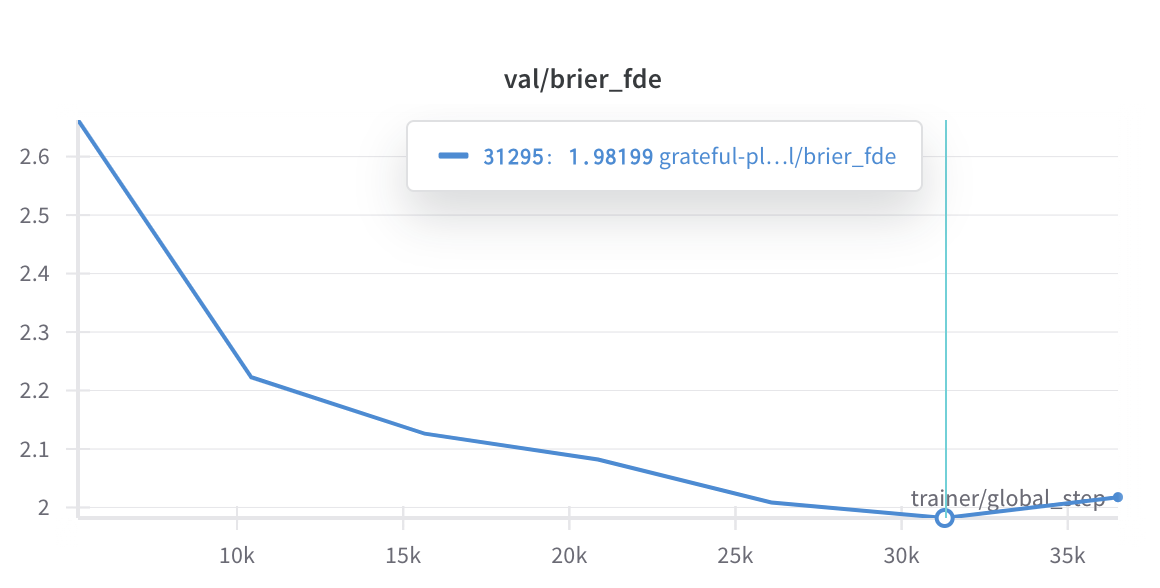
\includegraphics[clip, width=\textwidth]{figures/val_brier_fde.png}
        \caption{val/brier\_fde: 1.98199}
    \end{subfigure}
    \caption{Performance metrics on the validation set during MTR training. The plots show a consistent decrease in error for miss rate, FDE, ADE, and Brier-FDE as training progresses. }
    \label{fig:validation_metrics_merged}
\end{figure}

\subsubsubsection{Qualitative Analysis and Sample Case Illustration}
\label{sec:results_qualitative_merged}
% Detailed deconstruction of prediction examples (cf. presentation slides 10, 15 ), identifying ego agent, other agents, ground truth trajectories, and probabilistic forecasted paths. 
% Analysis of the influence of map topology (lanes, crosswalks) on predicted modalities. 
% Examination of model predictions in critical scenarios (e.g., agent behavior at intersections or pedestrian crossings), linking observed outputs to specific input features and model mechanisms. 
The qualitative analysis involves a detailed deconstruction of prediction examples. This process identifies the ego agent, other agents, ground truth trajectories, and the probabilistic forecasted paths generated by the model. The analysis also examines the influence of map topology, such as lanes and crosswalks, on the predicted modalities. Furthermore, it includes the examination of model predictions in critical scenarios, like agent behavior at intersections or pedestrian crossings, to link observed outputs to specific input features and model mechanisms.

Figure \ref{fig:mtr_prediction_merged} serves as a sample case, showing a multimodal prediction for a right-turn scenario. The model generates multiple future trajectories and assigns a probability to each. The green line represents the ground truth future path, while the colored lines show the model's predictions, with one having a much higher probability (p=0.36) than another (p=0.02).

% toDO(luroess): Generate new visualization for MTR prediction, this looks awful 
\begin{figure}[htbp]
    \centering
    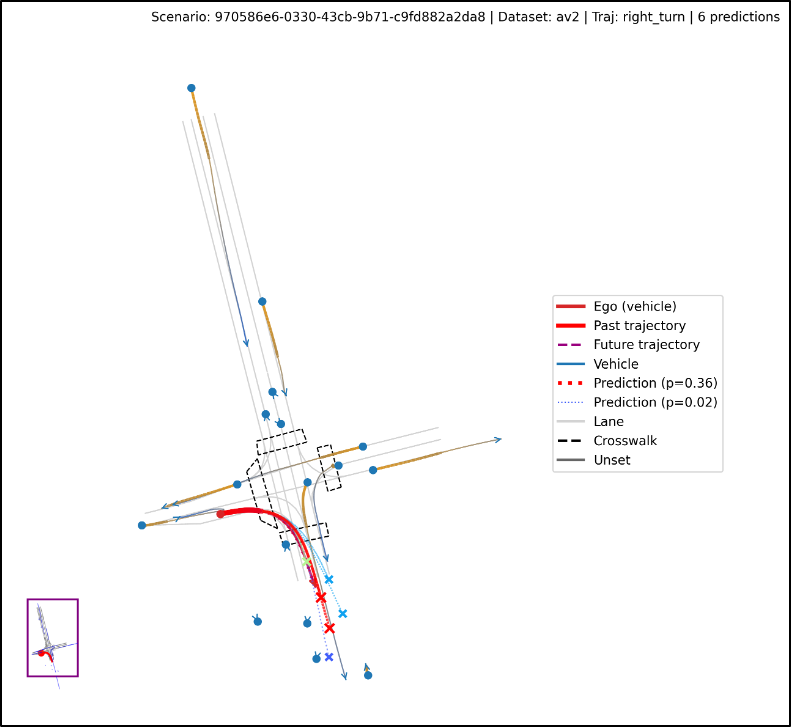
\includegraphics[width=0.8\textwidth]{figures/input_output_viz_ugly.png}
    \caption{A multimodal prediction from the MTR model for a right-turn scenario. The green line is the ground truth, and the colored lines are predictions with different probabilities.}
    \label{fig:mtr_prediction_merged}
\end{figure}